\begin{titlepage}
 
\begin{center}
 
 
% Upper part of the page
%
\includegraphics[width=0.7\textwidth]{jodcubelogo00}
%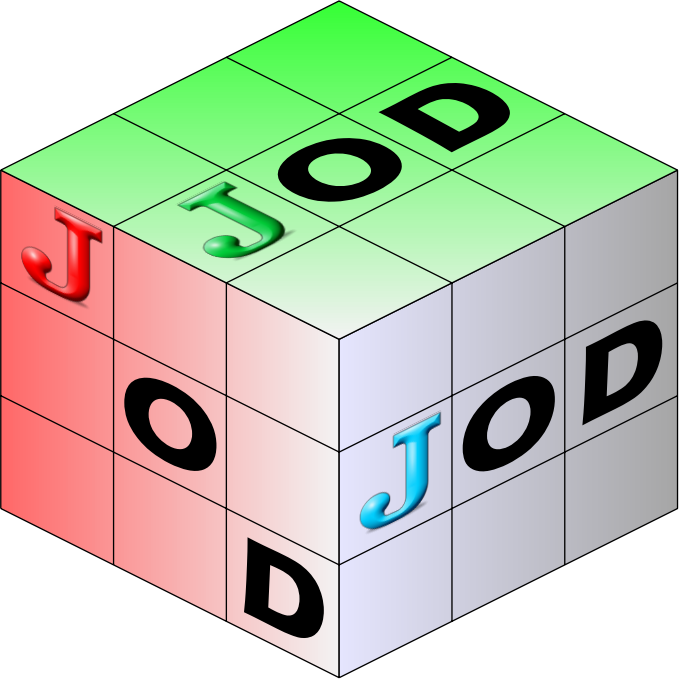
\includegraphics[width=0.7\textwidth]{jodcubelogo01} 
\href{http://bakerjd99.wordpress.com/the-jod-page/}{
\includegraphics[width=0.3\textwidth]{jodRGBcube}} 
 
% Title
\HRule \\[0.8cm]

{ \Huge \bfseries \jodred{J} \jodgreen{O}bject \jodblue{D}ictionary}\\[0.4cm]

\textsl{A code, test and documentation database system for J}\\[0.4cm]
 
\HRule \\[0.8cm]
 
 
% Author and supervisor
\begin{minipage}{0.4\textwidth}
\begin{flushleft}
\emph{Author:}\\
John D. Baker \\
\texttt{bakerjd99@gmail.com} \\
\end{flushleft}
\end{minipage}
\begin{minipage}{0.4\textwidth}
\begin{flushright}
\emph{Release:}\\
\jodversion \\
\today \\
\end{flushright}
\end{minipage}

\vspace{0.8cm}

\emph{Print dimensions: US Letter}

Bound printed version at \texttt{www.lulu.com}

%\jodurl{http://www.lulu.com/shop/john-baker/jod-j-object-dictionary/paperback/product-20076023.html}
\href{http://www.lulu.com/shop/john-baker/jod-j-object-dictionary/paperback/product-20076023.html}{Printed Version Link}

\begin{table}[ht]
  \centering
   \footnotesize
   %\rowcolors{0}{}{TableStripes}
   \begin{tabular}{|l|l|p{0.3\textwidth}|} \hline
      \multicolumn{3}{|c|}{\textbf{Document Version History}}\\ \hline
      \multicolumn{1}{|c|}{\textbf{Date}}  &
      \multicolumn{1}{c|}{\textbf{Version}} &
      \multicolumn{1}{|c|}{\textbf{Description}} \\ \hline\hline  
       \today              & \jodversion & current version  \\
       November 15, 2012   & 0.9.85      & JAL update \\ 
       April 21, 2012      & 0.9.75      & Lulu draft \\ 
       December 9, 2011    & 0.9.6       & Lulu draft \\
       November 30, 2011   & 0.9.5       & changed JOD logo \\ 
	    October 31, 2008    & 0.8.0       & first printed edition \\ 
       October 7, 2008     & 0.7.3       & first $\beta$ edition  \\ 
       September 24, 2008  & 0.7.1       & release draft \\
       August 18, 2008     & 0.6.0       & release draft \\
        \ldots             & \ldots      & \ldots \\
       %\multicolumn{1}{c}{\ldots} &  
       %\multicolumn{1}{c}{\ldots} & 
       %\multicolumn{1}{c}{\ldots}  \\ 
       March 30, 2008      &  0.3.5      & first draft \\ \hline
       \end{tabular}
	\caption{Document Version History}
	\label{tab:verhistory}
\end{table}
 

%\vfill 

% Bottom of the page
%{\large \today}
 
\end{center}
 
\end{titlepage}
